\documentclass[11pt]{jreport}
\usepackage{wuse_thesis}
\usepackage{indentfirst}
\usepackage{url}	% \url{}コマンド用.URLを表示する際に便利
\usepackage{xcolor} 	% 色を扱うためのパッケージ
\usepackage{listings}
\usepackage[dvipdfmx]{graphicx}
\usepackage{amsmath}
\usepackage{multirow}
\usepackage{array}
\usepackage{tabularx}
\usepackage{jvlisting}
% \usepackage{graphicx}  % ←graphicx.styを用いてEPSを取り込む場合有効にする
			% 他のパッケージ・スタイルを使う場合には適宜追加

% コード表示のカスタマイズ

\lstset{
  basicstyle={\ttfamily},
  identifierstyle={\small},
  commentstyle={\smallitshape},
  keywordstyle={\small\bfseries},
  ndkeywordstyle={\small},
  stringstyle={\small\ttfamily},
  frame={tb},
  breaklines=true,
  columns=[l]{fullflexible},
  numbers=left,
  xrightmargin=0zw,
  xleftmargin=3zw,
  numberstyle={\scriptsize},
  stepnumber=1,
  numbersep=1zw,
  lineskip=-0.5ex,
  keepspaces=true,           % スペースを保持
  language=Python,           % Python言語の指定
  texcl=true,               % TeXコマンドを有効化
  mathescape=true,          % 数式モードを有効化
  escapeinside={(*@}{@*)},
}
% ハイライト用の色定義(赤と緑)
\definecolor{highlightred}{rgb}{1.0, 0.8, 0.8} % 淡い赤
\definecolor{highlightgreen}{rgb}{0.8, 1.0, 0.8} % 淡い緑

\newcommand{\RQone}{コーディングパターンとして抽出すべき基準はどこなのか}
\newcommand{\RQtwo}{抽出したコーディングパターンはプロジェクトでどの程度使用されているのか}

\newcommand{\todo}[1]{\colorbox{yellow}{{\bf TODO}:}{\color{red} {\textbf{[#1]}}}}
\newcommand{\change}[1]{\colorbox{green}{{\bf CHANGE}:}{\color{blue} {\textbf{[#1]}}}}
\newcommand{\new}[1]{\colorbox{cyan}{{\bf NEW}:}{\color{black} {\textbf{[#1]}}}}

%%%%%%%%%%%%%%%%%%%%%%%%%%%%%%%%%%%%%%%%%%%%%%%%%%%%%%%%%%%%%%%%%%%%%%%%

%%
%% 主に表紙を作成するための情報
%%

%%  タイトル(修論の場合は英語表記も指定)
\title{プロジェクト特有のコーディングパターン\\収集方法の定量的評価}

%%  著者名(修論の場合は英語表記も指定)
\author{野口 朋弥}

%% 卒業論文
\bachelar	% 卒業論文(4年生用)

%%  学科・クラスタ
\department{システム工}

%%  学生番号
\studentid{60266227}

%%  卒業年度
\gyear{2024}		% 提出年が2022年なら,2021年度

%%  論文提出日∂
\date{2025年2月12日}	% 修士の場合は月(2021年2月)までとし,英語表記も指定
%\edate{February 2021}	% 修士の場合,こちら(英語表記)も有効化

%%%%%%%%%%%%%%%%%%%%%%%%%%%%%%%%%%%%%%%%%%%%%%%%%%%%%%%%%%%%%%%%%%%%%%%%

\begin{document}

\maketitle

%%
%%  概要
%%
\begin{abstract}
ソフトウェア開発において,開発効率の向上を目指して深層学習や正規表現などを利用したソースコードの自動生成の手法が多数提案されている.その多くは,GitHubやGerritなどのオープンソースプラットフォームで公開されている大規模なプロジェクトの開発履歴を学習データとして利用している.これらの手法は,多数のプロジェクトから関数やクラスの実装方法,APIの使用方法,エラーハンドリングなどの特徴を学習することで,特定のプログラミング言語における汎用的なソースコードの生成を実現している.

しかし,個別プロジェクトが定める規約やドメインによって,必ずしも汎用的なソースコードの実装が適切とは限らない.例えば,金融システムや医療システムといった重要インフラでは,セキュリティ要件や法的規制が厳格であり,独自のアーキテクチャ設計が不可欠となっている.また,複数人で開発を行う際のコーディング規約もプロジェクトごとに異なることがあるため,汎用的な生成手法では,ドメイン固有の要件を満たすソースコードを適切に生成できないことが多い.

従来研究では個別プロジェクトに特化したコーディングパターンを抽出する手法が提案されているが,実装方法全てをコーディングパターンとして抽出すると膨大になってしまい,その中にはプロジェクトの実装方法として現在は利用されていないものも含まれる.本研究では,個別のプロジェクトに特化したコーディングパターンを抽出する条件を提案する.これを元に,ソースコードの自動生成,自動修正手法に有用なパターンの収集手法を開発し,定量的に評価する.
\end{abstract}

%%  目次
\tableofcontents

%%  図目次 (図目次をいれたければ以下のコメントをはずす)
%\listoffigures

%%  表目次 (表目次をいれたければ以下のコメントをはずす)
%\listoftables

\newpage
\pagenumbering{arabic}	% 以降のページ番号を算用数字に

%%%%%%%%%%%%%%%%%%%%%%%%%%%%%%%%%%%%%%%%%%%%%%%%%%%%%%%%%%%%%%%%%%%%%%%%

%%
%%  本文はここから
%%
%%%%%%%%%%%%%%%%%%%%%%%%%%%%%%%%%%%%%%%%%%
\chapter{はじめに}
%%%%%%%%%%%%%%%%%%%%%%%%%%%%%%%%%%%%%%%%%%
昨今のソフトウェア開発では,開発効率の向上を目指した深層学習や正規表現などを利用したソースコードの自動生成,自動修正手法が多数提案されている\cite{deep_learnnig1}\cite{deep_learning2}\cite{deep_learnnig3}\cite{deep_learnning4}.
これらの手法の多くは,GitHub\footnote{GitHub:~\url{https://github.com}},Gerrit\footnote{Gerrit:~\url{https://www.gerritcodereview.com}}などでオープンソースソフトウェアとして公開されている大規模なプロジェクトの開発履歴を学習データとして利用している.GitHubには,数百万を超えるプロジェクトが公開されており,多様なプログラミング言語やコーディングスタイルで実装されたソースコードが蓄積されている.蓄積されたソースコードから,関数・クラスの実装方法や,APIの使用方法,エラーハンドリングなどの特徴を深層学習や正規表現によって形式化することで,ソースコードの自動生成,自動修正手法を実現している.また,開発履歴には再利用を容易にする実装パターンも多く含み,生成したソースコードの保守性や品質を担保するのに役立ち,長期的な保守や拡張を実現する.
%さらに,ソースコードの自動生成手法は,デザインパターンと呼ばれるソフトウェア設計の知識も学習に利用している.デザインパターンは,特定の問題に対する再利用可能な設計パターンを提供し,生成したソースコードの保守性や品質を担保するのに役立っている.
%これにより,自動生成されたコードが単に動作するだけでなく,長期的なメンテナンスや拡張が容易なものとなることが期待される.

しかし,個々のプロジェクトでは,ドメイン固有の要件が存在する.例えば,金融システムや医療システムといった重要インフラでは,セキュリティ要件や法的規制が厳格であり,独自のアーキテクチャ設計が不可欠となっている\cite{finacial}\cite{financial2}\cite{medical}.システムの利用場所の違いに限らず,コーディング規約といった複数人で開発を行う際にプログラミングにおける規則を定めたものでさえ,プロジェクトごとに異なることがあるため,汎用的な生成手法では,ドメイン固有の要件を満たすソースコードを適切に生成できないことも多い.

従来研究では,個別プロジェクトに特化した実装方法を再利用可能な形に抽象化したもの(以降コーディングパターン)を抽出する手法が提案されている\cite{devreplay}.しかし,実装方法全てをコーディングパターンとして抽出すると膨大になってしまい,その中にはプロジェクトの実装方法として現在は利用されていないコーディングパターンも多数含まれる.本研究では,個別のプロジェクトに特化したコーディングパターンを抽出する条件を提案する.これを元に,ソースコードの自動生成,自動修正手法に有用なパターンの収集手法を開発し,定量的に評価する.具体的には,2つのResearch Questions(RQ)に回答する.
\begin{itemize}
    \item RQ1: \RQone
    \item RQ2: \RQtwo
\end{itemize}

RQ1では,プロジェクトから生成された実装方法から,コーディングパターンとして含めるべき基準を分析し,
RQ2では,検出したコーディングパターンが出現する期間,その後も使用されているのかなどを分析することで,有用性の評価を行う.

以降,本論文では,\ref{sec:related}章でコーディングパターンと従来のデザインパターンの違いと,本研究の位置付けを述べ,\ref{sec:pattern}章では,プロジェクトの開発履歴から,変更差分を取得し,コーディングパターンになり得る候補を生成する手法について説明する.\ref{sec:dataset}章では本研究で使用するデータセット,\ref{sec:filter}章では抽出したコーディングパターン候補を述べ,\ref{sec:filter}章でRQ1,\ref{sec:time}章でRQ2のそれぞれの動機,手法,結果,考察について述べ,7章で本研究の妥当性について述べ,8章でまとめる.
% 多人数でソフトウェアを開発する場合,開発チーム全体であらかじめルールを共有することが重要である.共通のルールの導入により,開発効率の向上,ソフトウェア品質の改善,保守性の向上などが期待できる.\todo{引用}
% 開発チームで共有するルールの1例として,デザインパターンがある.
% デザインパターンとは,過去のソフトウェア設計者が発見し,編み出してきた設計のノウハウを体系的に蓄積し,再利用しやすい形式でまとめたものである.
% デザインパターンを活用することで,開発プロセスを効率化するとともに,設計の一貫性を保つことができる.\todo{引用}

% デザインパターンはプロジェクト全般で活用可能な汎用性を重視して設計されている.しかし,デザインパターンを採用するだけでは,個別のプロジェクトや開発チームごとの特性や要件を十分に反映することは難しい.
%%%%%%%%%%%%%%%%%%%%%%%%%%%%%%%%%%%%%%%%%%
\chapter{コーディングパターン}\label{sec:related}
%%%%%%%%%%%%%%%%%%%%%%%%%%%%%%%%%%%%%%%%%%
% \section{デザインパターン\todo{消すかもなのでまだ見ない}}
% 多人数でソフトウェアを開発する場合,ソフトウェアの開発効率,品質,保守性の向上はプロジェクト成功の鍵となる.これらの特性を高めるため,ソースコードの記述方法や構造を統一する基準としてデザインパターンが用いられる.
% デザインパターンは,ソフトウェア設計において繰り返し発生する問題に対する再利用可能な解法を,パターン名と設計原則に基づいて体系化したものである.特定のプログラミング言語やフレームワークに依存せず,様々な開発場面で適用可能である\todo{引用}

% 代表的なデザインパターンとして,GoF(Gang of Four)が提唱した23種類のパターンが知られる\cite{GoF}.
% これらは次の3つのパターンに分類できる.
% \begin{description}
%     \item[\textbf{生成}] オブジェクトの生成プロセスを抽象化し,システムが特定のクラスに依存しない柔軟な設計を実現するためのパターン(例: Factory Method, Singleton).
%     \item[\textbf{構造}] クラスやオブジェクトの構成や関係を整理し,柔軟なシステム構造を構築するためのパターン(例: Adapter, Composite).
%     \item[\textbf{振る舞い}] オブジェクト間の相互作用やアルゴリズムのカプセル化により,責任の分配や通信プロセスを最適化するためのパターン(例: Observer, Strategy).
% \end{description}
% \begin{description}
%     \item[\textbf{可読性}] 他の開発者が理解しやすいソースコードを記述すること.変数名や関数名を役割が直感的にわかるように命名することが推奨される.また,適切なコメントやインデントを使用することで,可読性を向上させる.
%     \item[\textbf{保守性}] ソースコードを継続的に管理する過程で,簡単に変更や修正を行えるかを指す.ソースコードの重複を避け,関数やモジュールを適切に分割することで,他の部分への影響を最小限に抑える.
%     \item[\textbf{パフォーマンス}] 適切なアルゴリズム,データ構造を選択することで,処理速度やメモリ使用量を最適化する.
% \end{description}
\section{コーディングパターン}
コーディングパターンは,各プロジェクトや開発チームの修正方法を再利用可能な形で抽象化し,ソースコードを形式化したものである.
一方,デザインパターンは,ソフトウェア設計において繰り返し発生する問題に対する再利用可能な解法を,パターン名と設計原則に基づいて体系化したもので.特定のプログラミング言語やフレームワークに依存せず,様々な開発場面で適用可能である\cite{GoF}.
両者の違いは,デザインパターンが設計レベルの汎用性を重視するのに対し,コーディングパターンは実装レベルでプロジェクトの特性を捉えることで,開発効率とソースコードの品質向上を目指す点にある.
本研究では,実装レベルのプロジェクトの特性を捉えることで,ドメイン固有の要件を満たす実装方法を抽出することを目指す.

\section{関連研究}
ソースコードの自動生成および自動修正に関する研究では,深層学習や正規表現を基盤としたアプローチが主流となっている.Smithらは深層学習を用いたプログラム解析において,ソースコードの構造的特徴とコンテキスト情報を統合的に扱うアプローチを提案している\cite{smith}.この研究では,ソースコードを単なるテキストとして扱うのではなく,抽象構文木ベースのニューラルネットワークを用いることで構造的・意味的特徴を保持しながら学習を行い,コード分類やクローン検出などのタスクにおいて従来手法を上回る性能を達成している.他にも,OpenAIが開発したChatGPT\footnote{ChatGPT:~\url{https://chatgpt.com}}は,大規模言語モデルを活用してプログラミング支援を行う新たなアプローチを示している.ChatGPTは自然言語による対話的なインターフェースを通じて,コード生成,デバッグ,リファクタリングなどの多様なプログラミングタスクをサポートし,開発者の生産性向上に貢献している.

しかし,これらの大規模なデータを学習した手法では,学習データに含まれていないドメイン固有の要件を満たすソースコードを適切に生成することが困難である.そのため,プロジェクト固有のコーディングパターンを抽出し,それを反映したソースコードの自動生成を目指す研究が複数存在する.

Dongsunらは,プロジェクトのソースコード修正履歴からコーディングパターンを学習し,自動的に修正を行うPAR(Pattern-based Automatic program Repair)を提案している\cite{AutomaticPatch}.この手法は従来手法に比べて,修正の精度や信頼性を向上させる可能性を示しており,実際に27件のバグ修正に成功した.


Zhangらは,PythonとJavaの構文を体系的に比較することで,9種類のPython独自のコーディングパターン(リスト内包表記など)を特定した\cite{idiom}.開発履歴の解析を通じて,頻出するPython独自のコーディングパターンに逸脱するソースコードを抽出する.
これにより,コードレビューの効率化とPythonらしいソースコードの品質向上に成功している.

Uedaらが開発したツールDevReplay\cite{devreplay}は,抽象構文木(AST)の差分解析に基づき,トークン単位で修正方法を収集する.その後,収集した修正方法を抽象化することにより,コーディングパターンを特定した.これにより,従来の静的解析ツールでは検出困難であったプロジェクト固有の特性に依存するコーディングパターン(例: プロジェクト独自の依存関係に関するもの)を抽出可能であった.

\section{動機}
Uedaらは,単一のプロジェクトの開発履歴から頻出する修正方法を抽象化することで,コーディングパターンを特定した.しかし,特定したコーディングパターンがプロジェクトの修正方法を反映しているかを十分に検証していない.その結果,従来手法では,不要なパターンが大量に生成される,または必要なパターンを取りこぼしているという課題がある.
本研究ではこれらの課題を解決するために,個別プロジェクトに特化したコーディングパターンを抽出する手法を提案するとともに,取得した修正方法から,有用なコーディングパターンを選別する評価基準の確立を目指す.

% \section{従来研究}
% 従来研究では,チームで定めたコーディングスタイルに準拠していないパッチを自動修正するために,ソフトウェアの開発履歴で頻出するソースコードの修正方法をパターンとして収集し,頻繁にコードレビューで指摘を受けるソースコードの修正方法を開発者に提示する手法が提案されている.\cite{AutomaticPatch}\cite{findBugs}\cite{Relntancer}\cite{don'tDIY}

% Uedaらは,頻繁に修正される修正方法を検出するためのツールDevReplayを開発している.当該手法は,開発履歴から頻出する修正方法をトークン単位でパターンとして収集することで,頻繁にコードレビューで指摘を受けるソースコードの修正方法を開発者に提示する.\cite{devreplay}
% 当該手法により,従来の静的解析ツールでは検出することが困難だったパターンも検出可能であった.
% しかし,単一プロジェクトの開発履歴が少ない場合,コーディングパターンを特定するのが困難になる.
% そのため,本研究では,複数のプロジェクトから開発履歴を収集し,パターンを生成することで,各プロジェクトにおけるコーディングパターンを特定するためのデータを補完することを目的とする.これにより,単一プロジェクトでは捉えきれないパターンを網羅し,より多様なコーディングパターンの特定を可能にする.

%%%%%%%%%%%%%%%%%%%%%%%%%%%%%%%%%%%%%%%%%%
\chapter{コーディングパターン候補の生成}\label{sec:pattern}
%%%%%%%%%%%%%%%%%%%%%%%%%%%%%%%%%%%%%%%%%%
\section{概要}
図\ref{fig:pattern}を用いて,本研究ではPython言語を対象にコーディングパターン候補を生成する手法を示す.本研究では,従来研究を踏襲し修正方法を表したコーディングパターンを抽出するために,コーディングパターンになり得る候補(コーディングパターン候補)を生成する.候補の中から有用なコーディングパターンを抽出する方法は\ref{sec:filter}章の手法で述べる.

図\ref{fig:pattern}で示す変更は,Python言語において加算を行う際に,変数\texttt{`a'}を2回記述する必要がなくなり,ソースコードをシンプルかつ明確に記述できるようにする変更である.
本研究では,このような変更チャンクから,次のようなコーディングパターンを抽出する方法を示す.

\colorbox{lightgray!50}{\texttt{VAR\_1}} \colorbox{lightgray!50}{\texttt{- =}} \colorbox{lightgray!50}{\texttt{- VAR\_1}} \colorbox{lightgray!50}{\texttt{- +}} \colorbox{lightgray!50}{\texttt{+ +=}} \colorbox{lightgray!50}{\texttt{VAR\_2}}

このコーディングパターンは変数`\texttt{a}'と`\texttt{b}'を用いた加算操作を形式化したパターンである.具体的には,変更チャンク内で削除が行われた`\texttt{=}',`\texttt{a}',`\texttt{+}'のトークンに接頭辞`\texttt{-}'を付与し,追加が行われた`\texttt{+=}'のトークンに接頭辞`\texttt{+}'を付与している.その後,変数`\texttt{a}'と`\texttt{b}'をそれぞれ`\texttt{VAR\_1}',`\texttt{VAR\_2}'に抽象化する.これらの変更により,変数名に依存しない形で変更チャンクを表現できる.

コーディングパターン候補は次の3つのステップで生成する.
\begin{description}
    \item[変更履歴の取得: ] プロジェクトの変更履歴を取得する.
    \item[前処理: ] 変更履歴から,修正前後のソースコードを抽出し,比較可能な形に整える. 
    \item[コーディングパターン候補の生成: ] 修正前後のチャンクを比較することで,修正方法から想定されるコーディングパターン候補を生成する.
\end{description}
% 本研究では,RQ1で単一のプロジェクトで生成されるパターン数の遷移を検証する.
% RQ2では,単一のプロジェクトに生成されるパターンと,複数プロジェクトのパターンがどれだけ有用なパターンであるかを検証する.
% RQ3では,従来手法ではパターンの生成が難しかったプロジェクトに対して,提案手法である複数プロジェクトからパターンを生成することで,プロジェクトにとって意味のあるパターンは増加したのかを検証する.

% 本研究では,以下の3つの手法でパターンを作成する.
% \begin{itemize}
%     \item 単一のプロジェクトからパターンを生成(従来手法)
%     \item データセットとして選択したプロジェクト全てからパターンを生成(提案手法)
%     \item データセットの中からコーディングパターンが似ていると思われるプロジェクトを選択し,パターンを生成(提案手法)
% \end{itemize}

% 提案手法において,複数プロジェクトからパターンを生成する理由は,開発履歴から作成されたパターンを適用できないソースコードの実装方法が存在する場合,実装方法として正しいかどうかをパターンから判断できない.
% そのため,複数のプロジェクトからパターンを生成し,パターン数を増やすことで,実装方法の正当性をパターンに基づいて判断できるケースを増加させることを目指す.

% 次に,コーディングパターンが似ていると思われるプロジェクトを選定して統合する理由について説明する.すべてのプロジェクトの開発履歴を用いる手法はパターン数を増加させることで,パターンが適用可能な実装方法を広げる効果が期待できる.しかし,この方法では生成されたパターンが特定のプロジェクトのコーディングパターンに沿った修正を保証するものではない.そのため,コーディングパターンが類似していると考えられるプロジェクトの開発履歴に限定して統合を行うことで,パターンの適用範囲を拡大し,正当性を向上させることを目指す.

\section{変更履歴の取得}\label{sec:get_change}
% 本手法では,コーディングパターン候補を生成するために,コードレビューによる修正箇所を分析対象とする.
% コードレビューでは開発者が変更したソースコードを複数人の別の開発者(検証者)が確認し,バグの修正や,組織の方針に従った実装になるよう指摘を行うため,本手法では組織の方針を捉えるためにコードレビューで変更されたソースコードを対象とする.

本研究では,コーディングパターン候補を生成するために,コードレビューを通じて修正された変更履歴を分析する.
コードレビューでは,開発者が変更したソースコードに対して,レビューアが確認を行い,バグの修正や組織の方針に従った実装となるように指摘を行う.そのため,組織の方針を把握するためには,コードレビューによって修正されたソースコードを分析することが適切である.

ここでは,コードレビューにおけるソースコードの変更を,パッチという単位で扱う.パッチとは,特定の時点におけるソースコードを示すものである.図\ref{fig:pattern}の上部に示すように,コードレビューのプロセスでは,開発者による最初の変更(\texttt{Patch\textsubscript{1}})と
から,レビューアの指摘に基づく修正を経て,最終的にプロジェクトに採択される変更(\texttt{Patch\textsubscript{n}})まで,複数のパッチが投稿される.

変更履歴の取得では,各ファイルについて,そのファイルが最初に編集されたパッチと,最後に修正されたパッチを特定する.具体的には,ファイルAが\texttt{Patch\textsubscript{1}}にて最初に編集され,\texttt{Patch\textsubscript{n}}にて最後に編集された場合,この2つのパッチを分析対象として取得する.また,別のファイルBでは,\texttt{Patch\textsubscript{2}}にて最初に編集され,\texttt{Patch\textsubscript{n-1}}にて最後に編集されているため,この2つのパッチを分析対象として取得する.このとき,一連のレビュープロセス(\texttt{Patch\textsubscript{1}}から\texttt{Patch\textsubscript{n}}の期間)にて修正が行われなかったファイルは,分析対象外とする.

\section{前処理}\label{sec: pre_process}
\ref{sec:get_change}節にて取得したパッチ単位のファイルから,ソースコードの具体的な変更内容を分析するために,変更チャンクを抽出する.変更チャンクとは,ファイル単位の差分から得られる追加行と削除行で構成される変更箇所を指す.このとき,文字の置換などの編集作業は,追加行と削除行の組み合わせとして表現される.

プロジェクトのコーディングパターンを正確に抽出するために,変更チャンクに含まれる非本質的な情報を除去し,本質的な変更のみを分析対象とする必要がある.そのため,次の3つの前処理を行う.
\begin{description}
    \item[コード注釈の削除:]プログラムの実行に影響を与えないコメント行(`\texttt{\#}'から始まる行)と関数やクラスの説明に利用される\texttt{docstring}を除去し,コーディングパターン生成に不要な情報を取り除く.
    \item[抽象化:]識別子や数値,文字列など具体的な表現を一般化(例:関数名をFUNCTION,変数名をVARなどに置換)することで,不要なノイズを低減し,汎化性能を向上させる.
    \item[変更チャンクの分割:]差分解析ツールであるGumTree\cite{gumtree}を用いて,取得した変更チャンクをより小さな変更チャンクに分割することで,変更の粒度を細かくし,パターン候補の生成効率を向上させる.
\end{description}
以下の各項で,これらの前処理の詳細と実装方法について説明する.
\subsection{コード注釈の削除}
コード注釈は,開発者間のソースコードの意図や使用方法を共有するために用いられる.しかし,これらはプログラムの実行には影響を与えないため,コーディングパターンの抽出において,不要な情報となる.そこで,コード注釈を削除する.

Listing\ref{list:comment}に,コード注釈を含むPythonのソースコード例を示す.このソースコードには,2種類のコード注釈が含まれる.1つは,`\texttt{\#}'から始まる行コメントであり,もう1つは\texttt{"""}で囲まれたdocstringである.docstringは,関数やクラスの概要,引数,戻り値などを体系的に記述するためのPythonの文章化機能である.これらのコード注釈は,ソースコードの可読性や保守性を向上させる重要な要素であるが,プログラムの実行ロジックには影響を与えない.そのため,コーディングパターンの抽出の際に,これらのコード注釈を全て削除する.


\begin{lstlisting}[caption=コード注釈の入ったソースコード,label=list:comment]
(*@\# 整数のリストを受け取り,各要素を2倍にする@*)
def double_numbers(numbers):
    (*@"""@*)
    (*@入力された数値のリストの各要素を2倍にする関数@*)
    
    (*@Args:@*)
    (*@    numbers: 整数のリスト@*)
    (*@Returns:@*)
    (*@    result: 2倍にした結果のリスト@*)
    (*@"""@*)
    result = []  (*@\# 結果を格納するリスト@*)
    for num in numbers:  (*@\# 各数値に対して処理@*)
        result.append(num * 2)
    return result
\end{lstlisting}

\subsection{抽象化}
プログラム自動修正の分野では,モデルの汎化性能を向上させるため,プログラム中の具体的な識別子やリテラルを抽象化することが一般的である.本研究においても,コーディングパターンの抽出精度を向上させるため,ソースコードの抽象化を行う.
しかし,本研究の目的は,プロジェクト固有の実装方法を抽出することにあるため,過度な抽象化はかえって有用な情報を失う可能性がある.そのため,以下に示す要素のみを抽象化の対象とする.
\begin{description}
    \item[関数名の抽象化] Pythonコードにおいて\texttt{def}キーワードによって定義された関数名を\texttt{FUNCTION}に置換する.複数の関数が存在する場合は,\texttt{FUNCTION\_1},\texttt{FUNCTION\_2}のように連番を付与して区別する.
    \item[識別子・数値・文字列の抽象化] 差分解析ツールGumTree\cite{gumtree}を用いて変更前後のコードの抽象構文木を生成し,対応する要素をマッチングする.そして,マッチした要素の種類に応じて,変数名などの識別子を\texttt{VAR}に,文字列リテラルを\texttt{STRING}に,数値を\texttt{NUMBER}に抽象化する.このとき,変更後のコードで新たに追加された識別子は,変更前のソースコードとマッチしないため抽象化されない.これにより,新規に導入された変数名や関数呼び出しなどの情報を保持することができる.
\end{description}

本手法による抽象化の具体例をListing\ref{list:A}からListing\ref{list:abst_B}に示す.
まず,Listing\ref{list:A}とListing\ref{list:B}はともに\texttt{def}キーワードによって関数\texttt{func}が定義されているため,これを\texttt{FUNCTION\_1}に抽象化する.
次に,両方のソースコードに共通して出現する引数\texttt{a}を\texttt{VAR\_1}に抽象化する.一方,Listing\ref{list:B}で新たに追加された引数\texttt{b}は,変更前のソースコードに対応する要素が存在しないため,抽象化されずにそのまま保持される.
これらの抽象化処理の結果,Listing\ref{list:A}はListing\ref{list:abst_A}に,Listing\ref{list:B}はListing\ref{list:abst_B}に変換される.

\begin{minipage}[b]{0.48\textwidth}
\begin{lstlisting}[caption=修正前ソースコード,label=list:A]
def func(a)
\end{lstlisting}
\end{minipage}
\begin{minipage}[b]{0.48\textwidth}
\begin{lstlisting}[caption=修正後ソースコード,label=list:B]
def func(a, b)
\end{lstlisting}
\end{minipage}


\begin{minipage}[b]{0.48\textwidth}
\begin{lstlisting}[caption=抽象化後の修正前ソースコード,label=list:abst_A]
def FUNCTION_1(VAR_1)
\end{lstlisting}
\end{minipage}
\begin{minipage}[b]{0.48\textwidth}
\begin{lstlisting}[caption=抽象化後の修正後ソースコード,label=list:abst_B]
def FUNCTION_1(VAR_1, b)
\end{lstlisting}
\end{minipage}

\subsection{変更チャンクの分割}
抽出した変更チャンクには,大規模な修正も含まれる.
大規模な修正をそのまま変更チャンクとしてパターン候補を生成すると,パターン候補生成のために使用するアルゴリズムの特性上,多大な時間がかかる.そのため,本手法では,変更チャンクを行単位で分割することで,処理時間の削減を図る.

変更チャンクを分割するために,GumTreeの解析結果を利用する.変更チャンクを抽象構文木で比較することで,変更位置を特定する.その後,置換操作が行われた行の開始位置を計算し,対応する行を別の変更チャンクとして分割する.

具体例をListing\ref{sp_src},Listing\ref{sp_dest}を用いて説明する.
この変更チャンクは,アサーション方法の変更が,3行にわたって行われている.
これらの修正を,GumTreeの変更位置の計算結果を元に,1行ごとに分割した変更チャンクに置き換える.

このように,変更チャンクを行単位で分割することで,変更の粒度を小さくし,パターン候補生成の効率化を実現している.

\begin{minipage}[b]{0.40\textwidth}
\begin{lstlisting}[caption=修正前ソースコード, label=sp_src]
assert expected == actual
assert expected2 == actual2
assert expected3 == actual3
\end{lstlisting}
\end{minipage}
\begin{minipage}[b]{0.50\textwidth}
\begin{lstlisting}[caption=修正後ソースコード, label=sp_dest]
self.assertEqual(expected, actual)
self.assertEqual(expected2, actual2)
self.assertEqual(expected3, actual3)
\end{lstlisting}
\end{minipage}
% \begin{description}
%     \item[コード注釈の削除:]ソースコードに含まれるコメント行(`\texttt{\#}'から始まる行)および,関数やクラスの説明に用いられる\texttt{docstring}を削除する.
%     \item[関数名の抽象化:] Pythonコードにおいて\texttt{def}キーワードによって定義された関数名を,\texttt{FUNCTION}という抽象的な識別子に置換する.
%     \item[識別子・数値・文字列の抽象化:] 変数名を\texttt{VAR},数値を\texttt{NUMBER},文字列を\texttt{STRING}にそれぞれ抽象化する.
%     \item[変更チャンクの分割: ] 差分解析ツールGumTree\cite{gumtree}を用いて,取得した変更チャンクをより細粒度の変更チャンクに分割する. 
% \end{description}
% それぞれの前処理について詳しく説明する.

% \noindent\textbf{[コード注釈の削除]}

% ソースコードに追加されたソースコードのチャンクから,変更された部分(以降,変更チャンク)を特定する.変更チャンクは,ファイル単位で差分を取得した際に得られる追加行と削除行から構成される.このとき,文字の置換なども追加と削除の組み合わせで表現する.

% 変更チャンクには,コメントの変更なども含まれるため,プロジェクトのコーディングパターンを反映した変更チャンクを収集するために前処理を行う.
% 前処理は次の3つを行う.
% \begin{description}
%     \item[コード注釈の削除:]ソースコードに含まれるコメント行(`\texttt{\#}'から始まる行)と関数やクラスの説明に利用される\texttt{docstring}を削除
%     \item[関数名の抽象化:]ソースコードに含まれる関数名(Pythonコードにおいて`\texttt{def}'によって定義されたもの)を`\texttt{FUNCTION}'に抽象化
%     \item[識別子・数値・文字列の抽象化:]変数名を`\texttt{VAR}',数値を`\texttt{NUMBER}',文字列を`\texttt{STRING}'に抽象化
%     \item[変更チャンクの分割:]差分解析ツールであるGumTree\cite{gumtree}を用いて,取得した変更チャンクをより小さな変更チャンクに変換
% \end{description}

\section{パターン候補の生成方法}\label{generate}
パターンの生成には系列パターンマイニング手法の1つであるPrefixSpan(Prefix-projected Sequential Pattern Mining)\cite{prefixspan}を用いる.PrefixSpanは効率的な系列パターンマイニング手法であり,順序を持つ系列データから頻出パターンを抽出する手法である.この手法を採用する理由は,変更チャンクに含まれるトークンの順序が,コード修正のパターンを表現する上で重要であるためである.
具体的なパターンの収集方法は,次の3ステップで構成される.
\begin{enumerate}
    \item 変更チャンクをトークン単位に分割し,変更前と変更後の差分情報を符号化する.変更前後のソースコードを比較した際に,変更により削除されたトークンに接頭辞`\textbf{-}',追加されたトークンには接頭辞`\textbf{+}'を付加する.この符号化により,変更操作のタイプ(追加・削除)を保持したトークン系列を生成することができる.
    \item トークン化された変更チャンクを,PrefixSpanの入力形式に適合するように変換する.変更前後のトークン列の順序関係を正確に表現するため,抽象構文木(AST)の構造に基づく差分解析手法を採用し,トークン間の意味的関連性を保持した系列表現を構築する.
    \item PrefixSpanアルゴリズムを適用し,頻出するトークン系列を抽出する.抽出されたパターン候補からは, 系列長が2未満のパターン,系列長が15以上のパターン,変更操作を示す符号(`\textbf{+}'/`\textbf{-}')を1つも含まないパターンを除外する.これにより,コード変更の文脈を反映した有意義なコーディングパターンのみを選定する.
\end{enumerate}
ここまでの手順で,コードレビューで行われた修正の特徴を抽象化したコーディングパターン候補を取得する.

% \section{パターンのフィルタリング方法}\label{filter}
% パターンの生成をしただけでは,冗長なパターンも含まれる.本研究では,3つのフィルタリングによって,冗長なパターンを削除する.
% \begin{itemize}
%     \item 変更を示唆しないパターンを削除する.変更を示唆しないパターンとは,パターンを構成するトークンに変更前と変更後のトークンが含まれないパターンである.
%     \item 重複するパターンを削除する.重複するパターンとは,パターンを構成するトークンが長いパターンの一部になっているパターンのことである.具体的には,図\ref{fig:create_pattern}に存在するパターン(\colorbox{lightgray}{\texttt{VAR\_1}} \colorbox{lightgray}{\texttt{=}})は,パターン(\colorbox{lightgray}{\texttt{VAR\_1}} \colorbox{lightgray}{\texttt{=}} \colorbox{lightgray}{\texttt{VAR\_1}})の一部とみなすことができるため,前者のパターンを重複したパターンとして削除する.
%     \item パターンを作成した開発履歴のデータセットにおいて,1度しか作成されなかったパターンを削除する.
% \end{itemize}
% 最後に各パターンの信頼度を式\ref{eq:confidence}を用いて算出する.
% 信頼度とは,パターンが適用可能なパッチに対して,パターンを適用することで正しい修正を行った割合を示す.

% %-------------------
% \begin{equation}\label{eq:confidence}
% \text{信頼度} = \frac{\text{パターンによって正しく変更されたパッチ数}}{\text{パターンが適用可能なパッチ数}}
% \end{equation}
% %-------------------
% 信頼度により,データセットにおいて各パターンによる修正の正確性を定量的に評価する.

%-------------------
\begin{figure}[h]
    \centering
        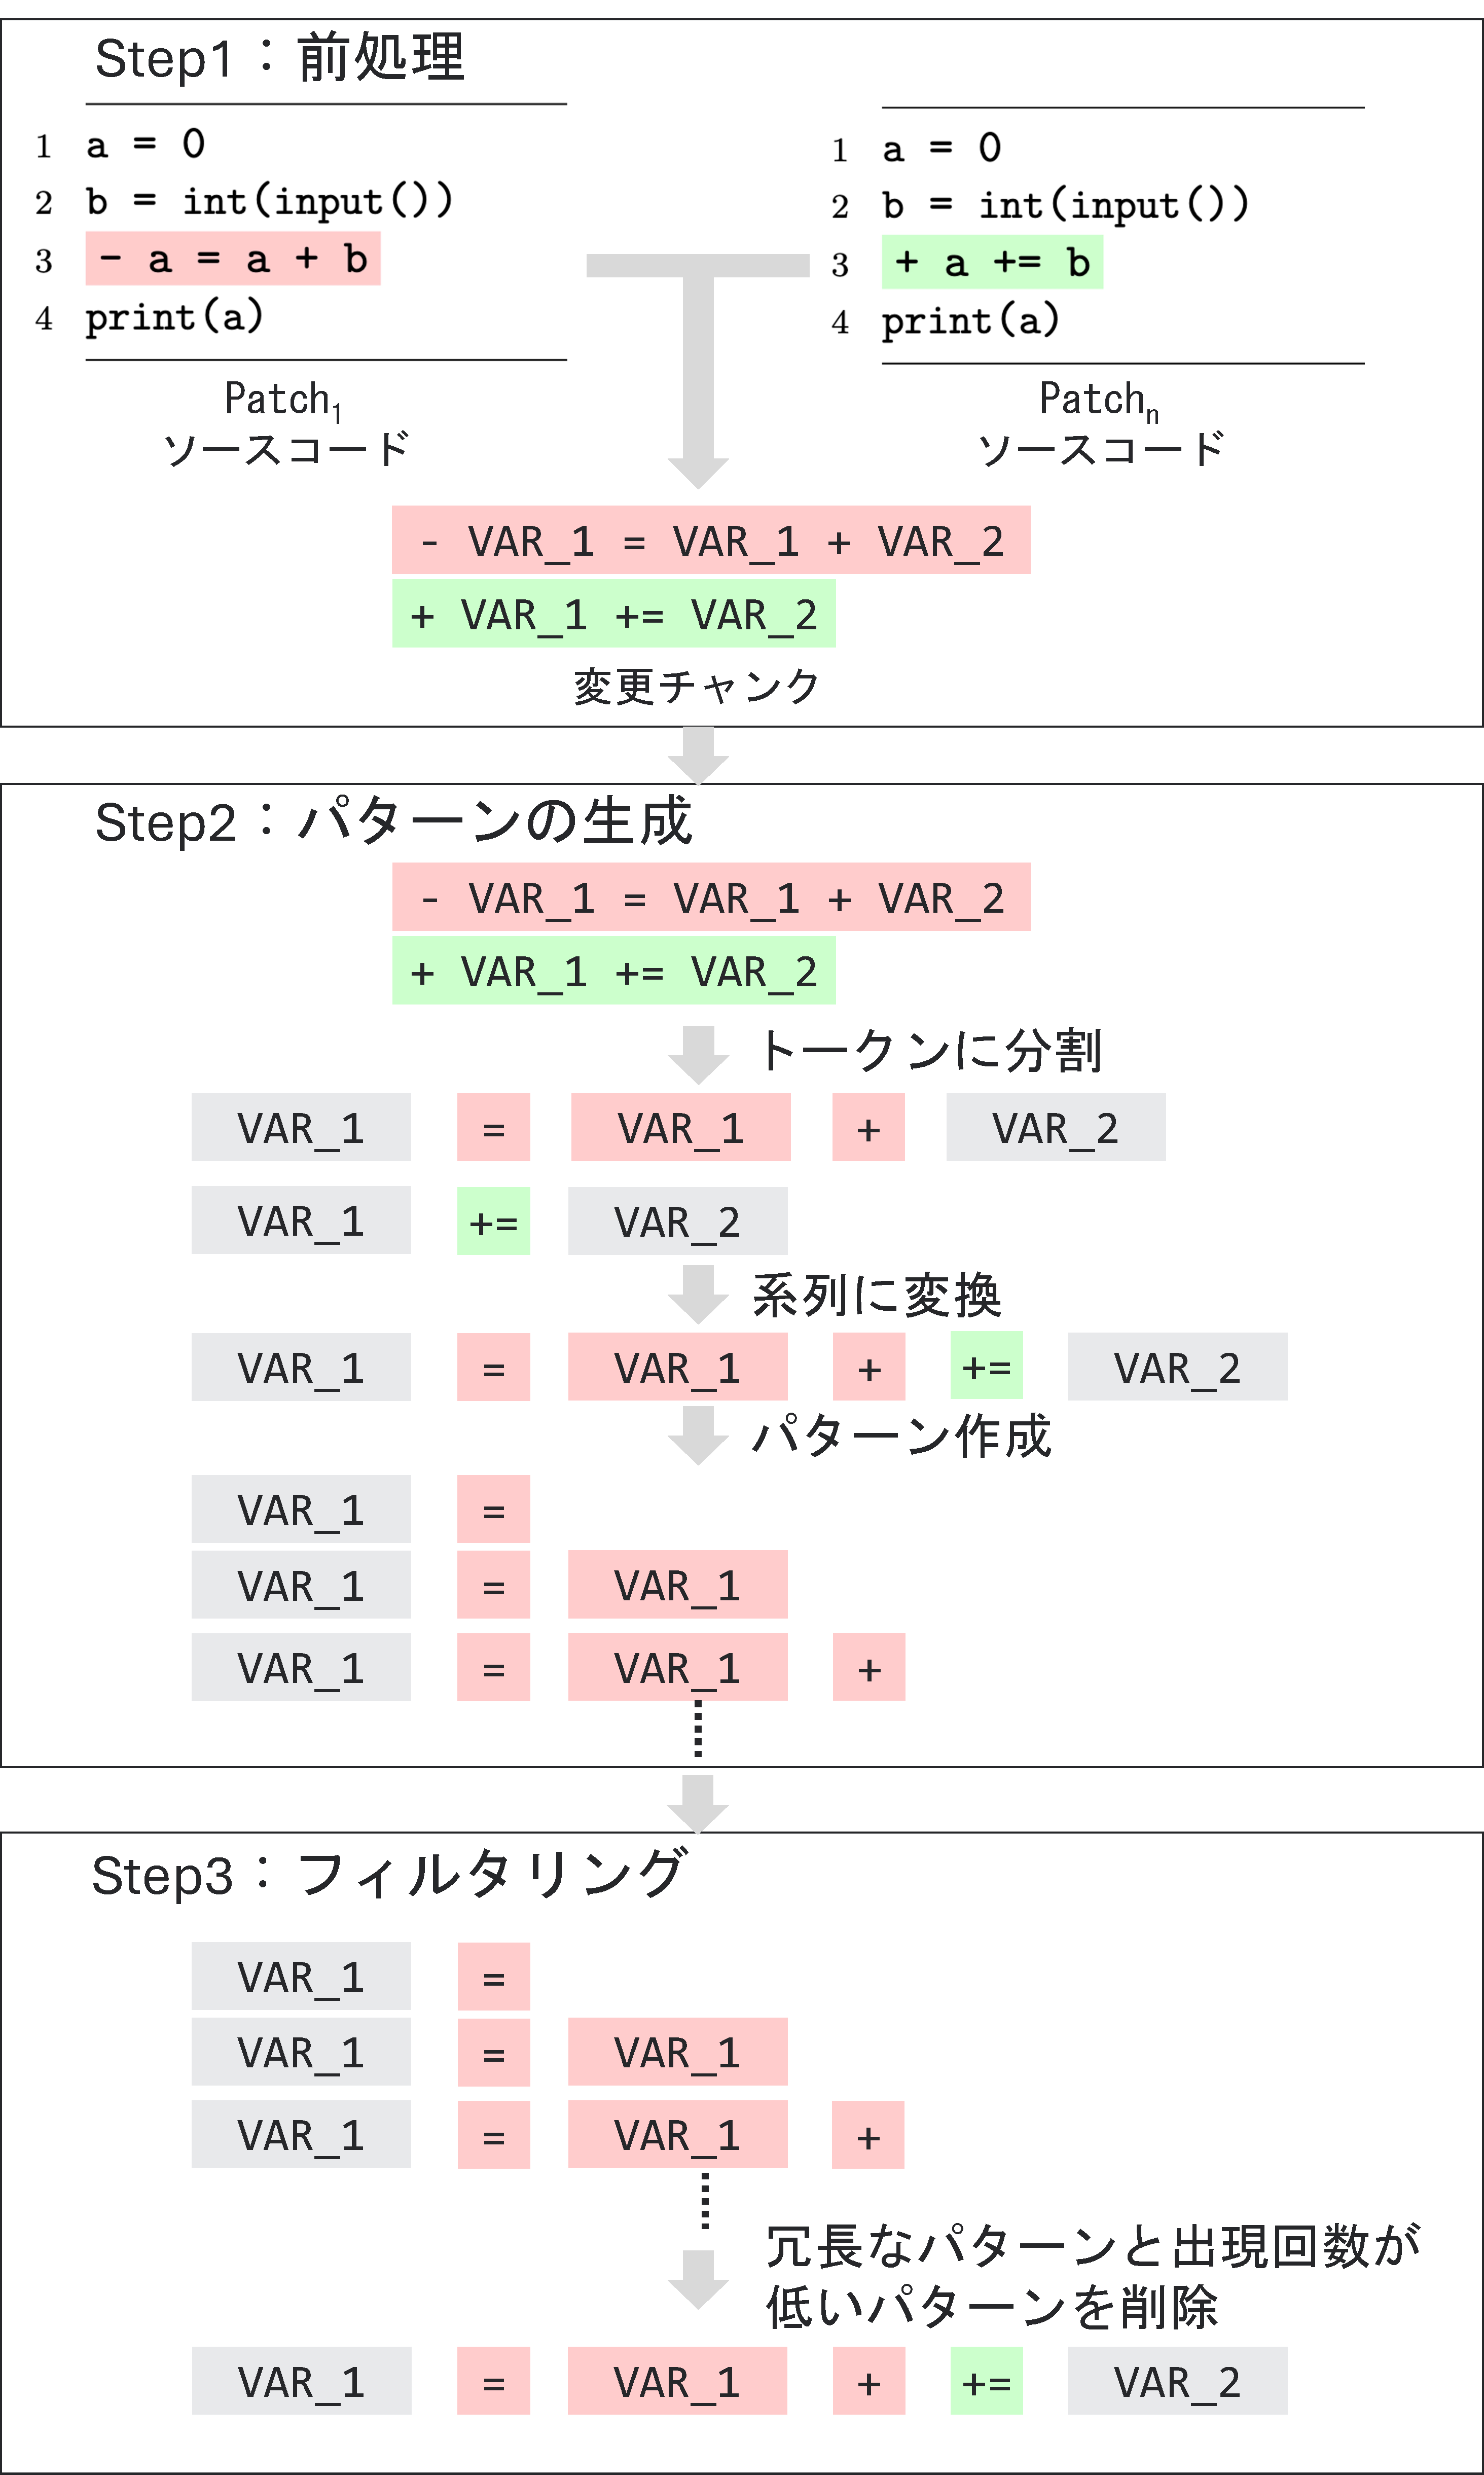
\includegraphics[width=1.0\linewidth]{@BSthesis2024_Noguchi/Noguchi_fig/create_pattern.pdf}
        \caption{コーディングパターン候補を生成するための概略図}
        \label{fig:pattern}
\end{figure}
%-------------------

%%%%%%%%%%%%%%%%%%%%%%%%%%%%%%%%%%%%%%%%%%
\chapter{データセット}\label{sec:dataset}
%%%%%%%%%%%%%%%%%%%%%%%%%%%%%%%%%%%%%%%%%%
\section{分析対象プロジェクト}
本研究では,ケーススタディとして大規模なオープンソースプロジェクトであるOpenStackのコンポーネントの中で最大規模のNovaを対象とした.Novaが分析対象として適切と判断した根拠は次の2点に基づく.
\begin{description}
    \item[規模的妥当性:]Open Infrastructure Fundationの技術レポート\cite{openstack}によると,Novaは2023年時点で約120万行のPythonコードを有しており,OpenStackプロジェクト群において最大の開発規模を有している.
    \item[開発プロセスの透明性:]OpenStackではレビュー管理システムとしてGerritを使用しており,各パッチに対するレビューアのコメント投稿数が多いため,レビューアの修正意図を反映したソースコードの変更差分が取得できる可能性が高い.
\end{description}

分析対象とする2013年1月1日から2025年1月1日までの9年間にmainブランチにマージされたコミットから,Python言語で記述されたファイルの変更差分を取得する.
データの収集方法は,mainブランチにマージされたパッチの履歴を抽出し,次の基準で取得する.
\begin{itemize}
    \item Pythonファイル(.py拡張子)に限定
    \item 変更が提案されたパッチと,mainにマージされたパッチに限定
\end{itemize}
本研究では,これらの基準で取得したパッチのファイル単位での変更差分について分析を行う.

\begin{table}[h]
    \centering
    \caption{データセットから抽出したコーディングパターン候補}
    \scalebox{1.1}{
    
        \label{table:not_filter_pattern}
        \begin{tabular}{r|c|r}
            \hline \hline
                順位 & パターン & 出現回数\\
            \hline
                 1 & \colorbox{lightgray!50}{\texttt{+ ,}} \colorbox{lightgray!50}{\texttt{)}} & 83,570 \\
                 2 & \colorbox{lightgray!50}{\texttt{(}} \colorbox{lightgray!50}{\texttt{+ ,}} & 65,253 \\
                 3 & \colorbox{lightgray!50}{\texttt{.}} \colorbox{lightgray!50}{\texttt{+ .}}     & 
                 53,093 \\
             \hline
        \end{tabular}
    }
\end{table}

\section{データセットから抽出したコーディングパターン候補}\label{subsec:difficult}
Novaプロジェクトを対象に,\ref{sec:pattern}章で説明した手法を用いてコーディングパターン候補を生成した結果を表\ref{table:not_filter_pattern}に示す.
出現頻度の高いパターンとして (\colorbox{lightgray!50}{\texttt{+ ,}} \colorbox{lightgray!50}{\texttt{)}}) のような形式が確認された.このような記号のみや括弧が閉じられていない不正な構造のパターンが,約2,790万件の候補のうち,約1,680万件(60.0\%)を占めた.

この傾向は,PrefixSpanのアルゴリズム特性に起因する.PrefixSpanのアルゴリズムは入力系列から全ての頻出部分系列を列挙するため,ソースコードとして文法的に不正なパターンであっても,出現頻度が閾値を超えていれば候補として抽出される.
例えば,`\textbf{,}'や`\textbf{.}'といったトークンは,関数呼び出し(例: \textbf{func(arg1, arg2)})やメソッドチェーン(例: \textbf{obj.method1().method2})など異なる文脈で高頻度に出現するため,必然的に出現頻度の高いパターンとして出力してしまう.

したがって,頻出するパターンの抽出だけではソースコードの文法的妥当性を保証したパターンを抽出することは困難である.
従来手法では,不適切なパターンを除外するための条件が提案されているが,その条件の妥当性に関する十分な議論はされていない.本来プロジェクトのコーディングパターンとして抽出すべきパターンが見逃される可能性がある.そのため,本研究では,\ref{sec:filter}章にて生成したコーディングパターン候補に対して,新たな選別条件を追加することで,より適切なプロジェクト固有のコーディングパターンの抽出を試みる.


%%%%%%%%%%%%%%%%%%%%%%%%%%%%%%%%%%%%%%%%%%
\chapter{RQ1:\RQone}\label{sec:filter}
%%%%%%%%%%%%%%%%%%%%%%%%%%%%%%%%%%%%%%%%%%
%フィルタリングに関するRQ
\section{動機}
\ref{subsec:difficult}節の分析結果から,コーディングパターン候補は膨大に生成されることが明らかになった.従来研究では,不適切なパターンを除外するための条件が提案されているが,その条件の妥当性に関する十分な検討がなされていない.その結果,プロジェクト固有のコーディングパターンが適切に抽出されない可能性がある.そのため,本研究では,プロジェクト特有のコーディングパターンを捉えるために,\ref{subsec:difficult}節の分析により判明した出現頻度の多かった不正な構造のパターンを排除し,従来手法より多くのプロジェクト固有のコーディングパターンを収集することを目指す.

\section{手法}
生成した候補からコーディングパターンとして抽出するために,従来研究で用いられていた条件を次に示す.

\textbf{従来研究の条件}
\begin{itemize}
    \item 変更を示さないパターンを削除する.具体的には,パターンの接頭辞に`\textbf{-}'と`\textbf{+}'が付加されたトークンの両方が含まれていないパターンを削除する.
    \item 重複した意味のパターンを削除する.具体的には,(\colorbox{lightgray!50}{\texttt{a}} \colorbox{lightgray!50}{\texttt{b}} \colorbox{lightgray!50}{\texttt{c}})というパターンと,(\colorbox{lightgray!50}{\texttt{a}} \colorbox{lightgray!50}{\texttt{b}})というパターンがあった場合,後者は前者の一部とみなすことができるため,後者のパターンは削除する.
\end{itemize}

これに対し,本研究では従来研究のパターンを次の3つの条件に変更する.

\textbf{提案手法の条件}
\begin{itemize}
    \item[条件1: ] 接頭辞に`\textbf{-}'と`\textbf{+}'が付加されたトークンが1つもないパターンを削除する.
    \item[条件2: ] 重複した意味のパターンを削除する.(従来研究と同じ)
    \item[条件3: ] 記号のみで構成されたパターンを削除する.
    \item[条件4: ] 括弧が閉じられていないパターンを削除する.
\end{itemize}

これらの条件を使用し,従来研究と本研究で抽出されたパターンを比較する.

\section{結果・考察}
表\ref{table:created_pattern}は,条件を適用しない場合,従来手法,および提案手法それぞれで抽出されたコーディングパターンの順位と出現回数を示している.また,表\ref{table:description}では,各パターンの具体的な内容と,そのパターンが適用される際の変更前後のソースコード例を示している.なお,表\ref{table:created_pattern}の順位において`\texttt{-}'は,その手法ではパターンとして抽出されなかったことを表している.約2,790万件のコーディングパターン候補を条件によって絞り込むと,従来手法では4,575件,提案手法では7,727件に集約することができた.従来研究であっても十分にコーディングパターン候補から絞り込むことができており,提案手法の方が絞り込みできていないようにも見える.具体的な内容について順に考察する.

条件1により,従来手法では変更を示さないパターンを除外し,提案手法では,変更を示すトークンが含まれないパターンを除外したことで,パターンとして取得する範囲が広くなったため,従来手法よりも3,000件ほど多くなった.取得する範囲が広くなったことにより,関数への引数追加/削除のようなパターンを取得することが可能になった.

しかし,抽出したパターンは,本研究の\ref{sec: pre_process}節の前処理の影響により,引数の追加/削除という操作の事実は把握できるものの,具体的なコーディングパターンの抽出が困難となる課題が確認された.この結果から,関数の引数変更に特化したパターン抽出を目的とする場合,関数名の抽象化は適切ではないと考えられる.関数名の抽象化を行わないことで,関数の引数を変更したという汎用的なパターンから,特定の関数に関する引数の追加をパターンとして抽出できるようになると考える.

条件2は,従来研究で用いられていた重複した意味のパターンを削除するという条件と同一のものである.この条件を適用することで,抽出したコーディングパターン候補の中から,似た意味のパターンを削除し,冗長なパターンを大幅に削除できた.

しかし,重複パターンを包括的に削除する手法には根本的な課題が存在する.具体例として,(\texttt{a = b + c})から(\texttt{a = b - c})への変更を上げる.この変更の本質は,`\texttt{+}'から`\texttt{-}'への置換であるが,行単位の差分解析では変更前後トークン列が(\colorbox{lightgray}{\texttt{a}} \colorbox{lightgray}{\texttt{=}} \colorbox{lightgray}{\texttt{b}} \colorbox{lightgray}{\texttt{- +}} \colorbox{lightgray}{\texttt{+ -}} \colorbox{lightgray}{\texttt{c}})という冗長な形式に集約されてしまう.重複削除処理により,本来抽出すべき演算子変更の核心パターン(\colorbox{lightgray}{\texttt{- +}} \colorbox{lightgray}{\texttt{+ -}})が失われ,冗長な行単位パターンだけが残存するという問題が発生する.

これを解決するための今後の課題として,抽象構文木(AST)を用いた差分解析手法の導入が考えられる.具体的には,AST同士を比較することで部分木の変更を検出し,その変更内容から適切なトークン列を生成する.この手法により,行単位の解析では捉えきれなかった演算子の変更や構文レベルのパターンも正確に抽出できる可能性がある.結果として,より意味的に妥当なコーディングパターンの抽出が期待され,冗長なパターンが削減されるだけでなく,プロジェクト固有のコーディングパターンの特定精度が向上する可能性がある.

また,条件3,4を利用することで,候補を生成する段階で出現頻度が高かった(\colorbox{lightgray}{\texttt{+,}} \colorbox{lightgray}{\texttt{)}})のようなソースコードの文法的に誤ったパターンを除外することができた.従来手法で抽出されたパターンには,頻出パターンの中で条件3,4を追加することで絞り込めるものは少なかったが,発生頻度が低いパターンには条件に合致するパターンも見られた.従って,これらの条件は頻出したパターン候補だけを対象にするのではなく,すべての抽出されたパターンを分析する場合において有用であると言える.
%-------------------
\begin{table}[t]
    \centering
        \caption{条件ごとにパターンを抽出した結果}
        \label{table:created_pattern}
        \begin{tabular}{r|rrr|r|l}
            \hline \hline
                \multirow{2}{*}{id} & \multicolumn{3}{c|}{順位} & \multirow{2}{*}{\begin{tabular}{c} 出現\\回数 \end{tabular}} & \multirow{2}{*}{説明} \\ \cline{2-4}
                
                & 条件なし & 従来 & 提案 & \\ 
            \hline
                 1 & 4,068      & 1   & 1  & 2,504  & 画像メタデータをオブジェクトとして渡すように変更\\
                 2 & 26,738    & -   & 2  & 1,067  & デコレータの名前・引数の変更\\
                 3 & 54,081    & -   & 3  & 975    & デコレータへの引数の追加\\
                 4 & 23,974    & 2   & -  & 1,311  & ログメッセージのローカライズ\\
                 5 & 75,393    & 3   & 4  & 756    & DB操作のリトライ処理をライブラリ化\\
                 6 & 1,201,923 & -   & -  & 110    & uuidを呼び出す処理の関数化\\
             \hline
        \end{tabular}
\end{table}
%-------------------
%-------------------
\begin{table}[t]
    \centering
    \caption{抽出したパターンの詳細}
    \label{table:description}
    \begin{tabular}{r|p{5cm}|p{4.5cm}|p{4.5cm}}
    % \begin{tabularx}{\textwidth}{r|X|>{\hsize=0.8\hsize}X|>{\hsize=0.8\hsize}X}
        \hline \hline
        id & パターン & 変更前ソースコード例 & 変更後ソースコード例 \\ \hline
        1 & 
        \colorbox{lightgray!50}{\texttt{VAR\_1}} \colorbox{lightgray!50}{\texttt{=}} \colorbox{lightgray!50}{\texttt{- \{}} \colorbox{lightgray!50}{\texttt{+ objects}} 
        \newline
        \colorbox{lightgray!50}{\texttt{+ .}} \colorbox{lightgray!50}{\texttt{+ ImageMeta}} \colorbox{lightgray!50}{\texttt{+ ,}} 
        \newline
        \colorbox{lightgray!50}{\texttt{+ from\_dict}} \colorbox{lightgray!50}{\texttt{+ (}} \colorbox{lightgray!50}{\texttt{+ self}} 
        \newline
        \colorbox{lightgray!50}{\texttt{+ .}} \colorbox{lightgray!50}{\texttt{+ test\_VAR\_1}} \colorbox{lightgray!50}{\texttt{+ )}}
        & 
        \texttt{image\_meta = \{\}} 
        & 
        \texttt{image\_meta = \newline
        objects.ImageMeta.from\_dict \newline
        (self.test\_image\_meta)} \\
        \hline
        2 &
        \colorbox{lightgray!50}{\texttt{@}} \colorbox{lightgray!50}{\texttt{- exception}} \colorbox{lightgray!50}{\texttt{- .}} 
        \newline
        \colorbox{lightgray!50}{\texttt{wrap\_exception}}
        \colorbox{lightgray!50}{\texttt{= (}} 
        \newline
        \colorbox{lightgray!50}{\texttt{- notifier}} 
        \colorbox{lightgray!50}{\texttt{- =}} 
        \newline
        \colorbox{lightgray!50}{\texttt{- notifier}} \colorbox{lightgray!50}{\texttt{- ,}}
        \newline
        \colorbox{lightgray!50}{\texttt{- publisher\_id}} \colorbox{lightgray!50}{\texttt{- =}} 
        \newline
        \colorbox{lightgray!50}{\texttt{- publisher\_id}} \colorbox{lightgray!50}{\texttt{- (}} \colorbox{lightgray!50}{\texttt{- )}} \colorbox{lightgray!50}{\texttt{= )}}
        &
        \texttt{@exception.
        \newline
        wrap\_exception
        \newline
        (notifier=notifier, publisher\_id=
        \newline
        publisher\_id())}
        &
        \texttt{@wrap\_exception()}\\
        \hline
        3 &
        \colorbox{lightgray!50}{\texttt{@}} \colorbox{lightgray!50}{\texttt{wrap\_instance\_event}} 
        \newline
        \colorbox{lightgray!50}{\texttt{+ (}} \colorbox{lightgray!50}{\texttt{+ prefix}} \colorbox{lightgray!50}{\texttt{+ =}} 
        \newline
        \colorbox{lightgray!50}{\texttt{+ compute}} \colorbox{lightgray!50}{\texttt{+ )}}
        &
        \texttt{@wrap\_instance\_event}
        &
        \texttt{@wrap\_instance\_event\newline
        (prefix = 'compute')}\\
        \hline
        4 &
        \colorbox{lightgray!50}{\texttt{VAR\_1}} \colorbox{lightgray!50}{\texttt{.}} \colorbox{lightgray!50}{\texttt{VAR\_2}} \colorbox{lightgray!50}{\texttt{(}}
        \newline
        \colorbox{lightgray!50}{\texttt{- VAR\_3}} \colorbox{lightgray!50}{\texttt{+ VAR\_4}}
        \colorbox{lightgray!50}{\texttt{(}}
        &
        \texttt{LOG.info(\_(}
        &
        \texttt{LOG.info(\_LI(}\\
        \hline
        5 &
        \colorbox{lightgray!50}{\texttt{@}} \colorbox{lightgray!50}{\texttt{- \_retry\_on\_deadlock}} 
        \newline
        \colorbox{lightgray!50}{\texttt{+ oslo\_db\_api}} \colorbox{lightgray!50}{\texttt{+ .}}
        \newline
        \colorbox{lightgray!50}{\texttt{+ wrap\_db\_retry}} \colorbox{lightgray!50}{\texttt{+ (}}
        \newline
        \colorbox{lightgray!50}{\texttt{+ max\_retries}} \colorbox{lightgray!50}{\texttt{+ =}} 
        \colorbox{lightgray!50}{\texttt{+ 5}} 
        \newline
        \colorbox{lightgray!50}{\texttt{+ ,}} \colorbox{lightgray!50}{\texttt{+ retry\_on\_deadlock}} 
        \newline
        \colorbox{lightgray!50}{\texttt{+ =}} \colorbox{lightgray!50}{\texttt{+ True}} \colorbox{lightgray!50}{\texttt{+ )}}
        &
        \texttt{@\_retry\_on\_deadlock}
        &
        \texttt{@oslo\_db\_api.wrap\_db\_retry
        \newline
        max\_retries=5, 
        \newline
         retry\_on\_deadlock=True)}\\
        \hline
        6 &
        \colorbox{lightgray!50}{\texttt{- str}} \colorbox{lightgray!50}{\texttt{- (}} \colorbox{lightgray!50}{\texttt{- uuid}} 
        \newline
        \colorbox{lightgray!50}{\texttt{+ uuidutils}} \colorbox{lightgray!50}{\texttt{.}} \colorbox{lightgray!50}{\texttt{- uuid4}} 
        \newline
        \colorbox{lightgray!50}{\texttt{+ generate\_uuid}} \colorbox{lightgray!50}{\texttt{= (}} 
        \colorbox{lightgray!50}{\texttt{= )}} \colorbox{lightgray!50}{\texttt{- )}}
        &
        \texttt{str(uuid.uuid4())}
        &
        \texttt{str(uuidutils.
        \newline
        generate\_uuid())}\\
        \hline
    \end{tabular}
\end{table}
% %-------------------
% \begin{table}[t]
%     \centering
%     % \caption{Caption}
%     \begin{tabularx}{\textwidth}{r|X|X}
%         \hline \hline
%         id & 変更前パターン & 変更後パターン \\ \hline
%         1 & 
%         VAR\_1 = \{\} 
%         &
%         VAR\_1 = objects.ImageMeta.\newline
%         from\_dict(self.test\_VAR\_1)\\
%         \hline
%         2 &
%         @exception.wrap\_exception(notifier = \newline
%         notifier, publisher\_id = publisher\_id()) 
%         &
%         @wrap\_exception()\\
%     \end{tabularx}
% \end{table}

% \begin{table}[t]
%     \centering
%     % \caption{Caption}
%     \begin{tabularx}{\textwidth}{r|X}
%         \hline \hline
%         id & パターン \\ \hline
%         1 &
%         \texttt{VAR\_1} = \colorbox{red!30}{\texttt{\{\}}} 
%         \colorbox{green!30}{\texttt{objects.ImageMeta.from\_dict(self.test\_VAR\_1)}}\\
%         \hline
%         2 &
%         \texttt{@}\colorbox{red!30}{exception.}\texttt{wrap\_exception(}
%         \colorbox{red!30}{\texttt{- notifier = notifier, publisher\_id = publisher\_id}}\texttt{)}
%     \end{tabularx}
% \end{table}
%%%%%%%%%%%%%%%%%%%%%%%%%%%%%%%%%%%%%%%%%%
\chapter{RQ2:\RQtwo}\label{sec:time}
%%%%%%%%%%%%%%%%%%%%%%%%%%%%%%%%%%%%%%%%%%
%時系列で何個かのパターン見た時の評価
\section{動機}
\ref{sec:filter}章の分析結果から,パターン候補に条件を設定することで,頻出するプロジェクトのコーディングパターンを反映したソースコードを特定した.しかし,Uedaらの従来研究\cite{devreplay}において,抽出されたコーディングパターンは時間経過に伴い使用頻度が変動することが明らかになっている.
このことから,抽出されたパターンには,以下のような特徴が存在すると考えられる.
\begin{itemize}
    \item コーディングパターンによる修正が行われる前のソースコード(以降,変更前パターン)が標準的な実装として採用されるケース
    \item 現在もコーディングパターンによる修正が行われたソースコード(以降,変更後パターン)が継続的に使用されているケース
    \item 過去には頻繁に使用されていた変更後パターンが,現在では使用されなくなったケース
\end{itemize}
本研究では,RQ1において抽出したコーディングパターンの生存期間を分析することで,長期間にわたって使用されるコーディングパターンと,比較的短期間で使用されなくなるコーディングパターンの特徴を明らかにする.この分析を通じて,プロジェクトにおけるコーディングパターンの持続性を評価し,効果的なコーディングパターンの収集手法の確立を目指す.

\section{手法}
本研究では,\ref{sec:filter}章にて抽出したコーディングパターンid\_1からid\_6を対象として時系列分析を行う.分析は次の手順にて行う.
\begin{itemize}
    \item NovaプロジェクトのGitリポジトリから,2013年から2025年までの各年1月1日時点にリポジトリに含まれるソースコードを取得する.
    \item 各スナップショットに対して,変更前パターンと変更後パターンが出現した回数を記録する.
\end{itemize}

\section{結果・考察}
図\ref{table:id_1},図\ref{table:id_2},図\ref{table:id_3},図\ref{table:id_5},図\ref{table:id_6},図\ref{table:id_4}は,id\_1からid\_6までの6つのパターンに対して時系列分析を行った結果を示す.横軸は取得したスナップショットの年数,縦軸は変更前/変更後パターンが出現した回数を示す.図中の黒色の棒グラフは,変更前パターンが抽出された数,白色の棒グラフは変更後パターンが出現した数を示す.id\_1は変更前/変更後パターンの両方が全期間で使用され,id\_2,id\_3,id\_5,id\_6のパターンはある時点を境に,変更後パターンしか使用されなくなり,id\_4はある地点以降は変更前/変更後パターンが両方使用されなくなった.
6つのパターンから,次の3つの特徴的な傾向を考察する
\begin{description}
    \item[持続的共存型パターン(id\_1)]: 分析期間を通じて,変更前/変更後パターンが継続的に共存している.
    \item[移行完了型パターン(id\_2,id\_3,id\_5,id\_6)]: 特定の時点を境に,変更前パターンが完全に変更後パターンに置き換えられた.
    \item[消失型パターン(id\_4)]: ある時点で,変更前/変更後パターンが出現しなくなった.
\end{description}

\noindent\textbf{[持続共存型パターン]} 
\begin{figure}[h]
    \centering
        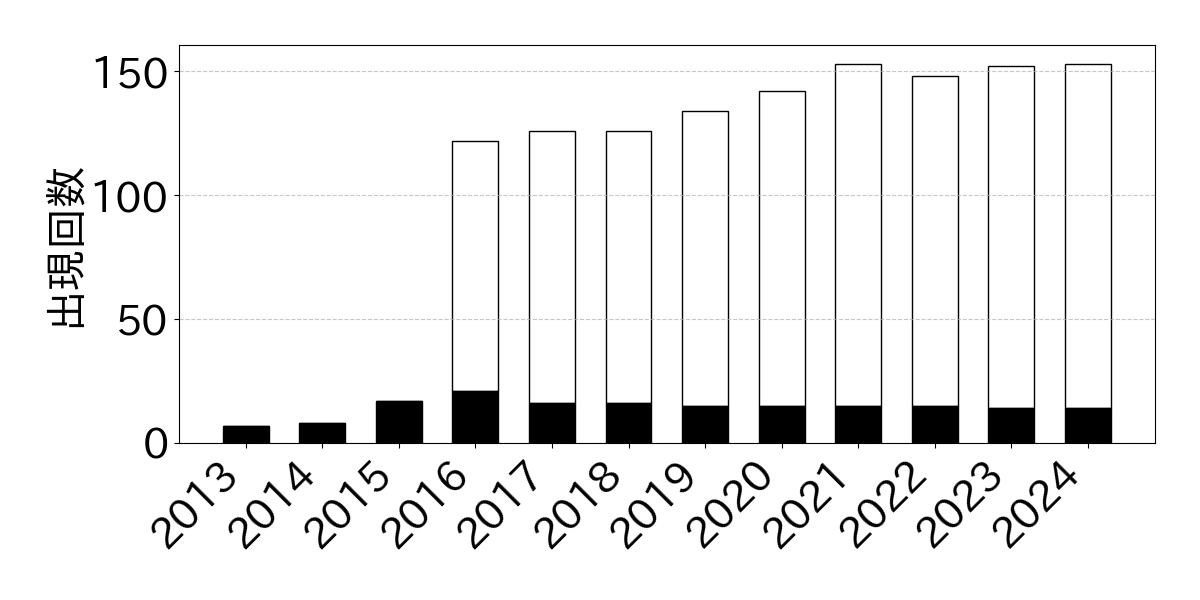
\includegraphics[width=0.8\linewidth]{@BSthesis2024_Noguchi/Noguchi_fig/id_1.png}
        \vspace{-4mm}
        \caption{id\_1のパターン}
        \label{table:id_1}
        
    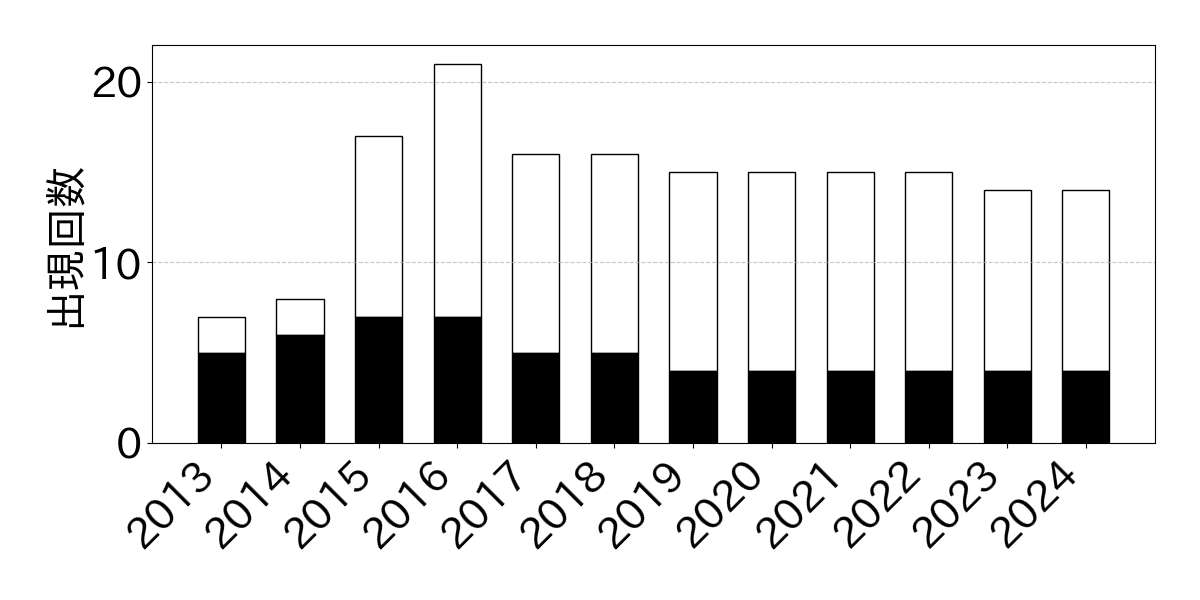
\includegraphics[width=0.8\linewidth]{@BSthesis2024_Noguchi/Noguchi_fig/test_or_not_test.png}
    \vspace{-4mm}
    \caption{id\_1の変更前パターンの内訳}
    \label{figure:test_or_not}
\end{figure}

当該パターンは,変更前/変更後パターンが継続的に共存している.id\_1のパターンは,テストの信頼性向上を目的として,テストデータをダミーデータからより具体的なオブジェクトに変更するものである.このパターンは,テストの品質向上を意図した変更であるにもかかわらず,変更前のパターンも引き続き使用されている.そのため,変更前パターンが引き続き使用されている理由について分析を行う.
このパターンはテストの信頼性向上を目的とした変更であることから,変更前パターンの出現箇所をテストコードと非テストコードに分類して分析を行った.その結果を図\ref{figure:test_or_not}に示す.
横軸は取得したスナップショットの年数,縦軸はテスト/テスト以外のコードで変更前パターンが出現した回数を示す.黒色の棒グラフがテストコード以外で出現した回数,白色の棒グラフがテストコードで出現した回数である.

図\ref{figure:test_or_not}の黒色の棒グラフを参照すると,テストコード以外で変更前パターンが出現した回数は,2019年から4件であり,変更前パターンが出現した箇所を分析すると同様の箇所であった.2019年以降で使用されたソースコードの内訳は,適用後のオブジェクトを定義した箇所,保守がなされていない箇所,後々のために残さざるを得なかった箇所,推奨されない関数内で使われている箇所の4つである.
テストコードで変更前パターンが出現した箇所では,\texttt{image\_meta}がオブジェクト型として入力されることを期待しているが,単体テストでは\texttt{image\_meta}が空でも動作するため,空の辞書で定義しているものであった.そのため,持続共存型のパターンは,保守がされていないパターン,または限定的に使用できるパターンで,今回の場合,テスト内では使用するべきパターンである.

\noindent\textbf{[移行完了型パターン] }

\begin{figure}[h]
    \centering
        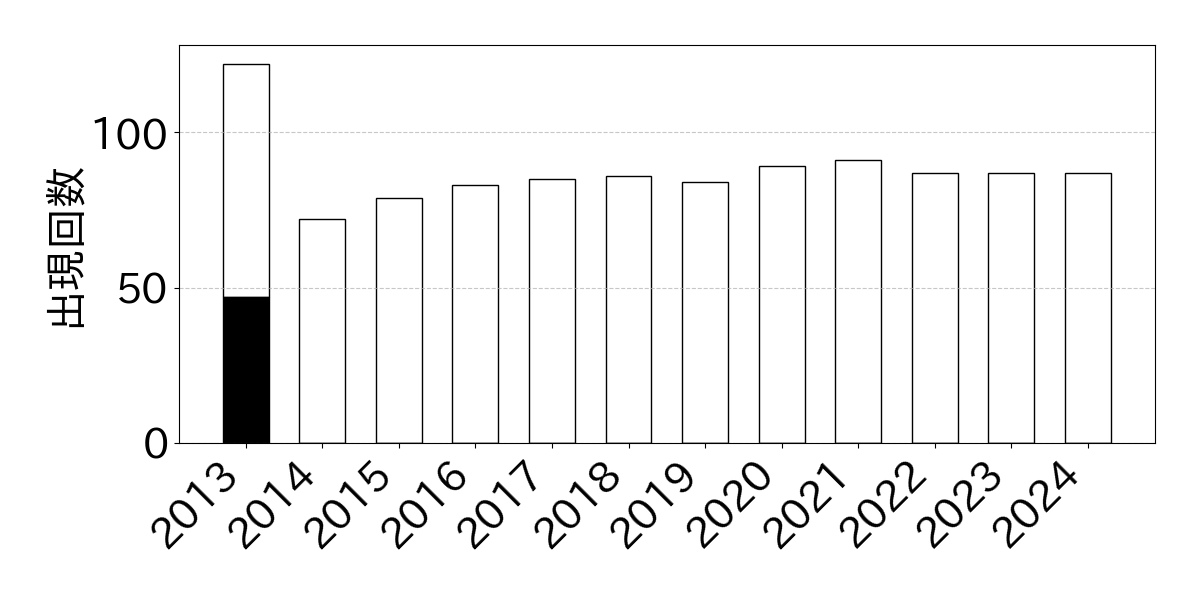
\includegraphics[width=0.8\linewidth]{@BSthesis2024_Noguchi/Noguchi_fig/id_2.png}
        \vspace{-4mm}
        \caption{id\_2のパターン}
        \label{table:id_2}
        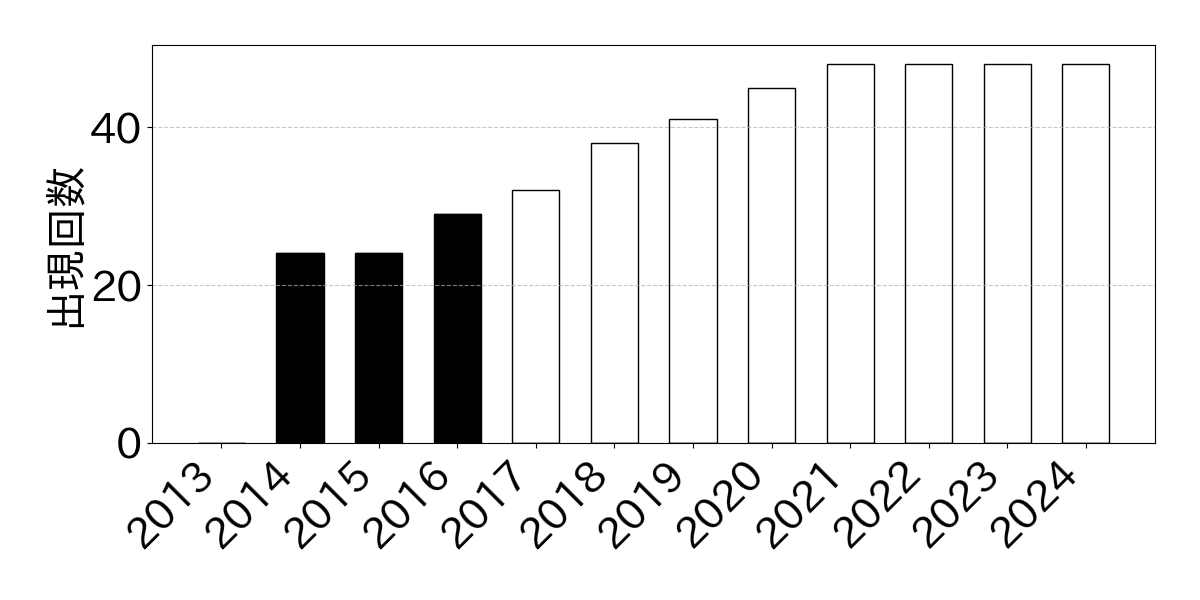
\includegraphics[width=0.8\linewidth]{@BSthesis2024_Noguchi/Noguchi_fig/id_3.png}
        \vspace{-2mm}
        \caption{id\_3のパターン}
        \label{table:id_3}
\end{figure}
\begin{figure}[h]
    \centering
        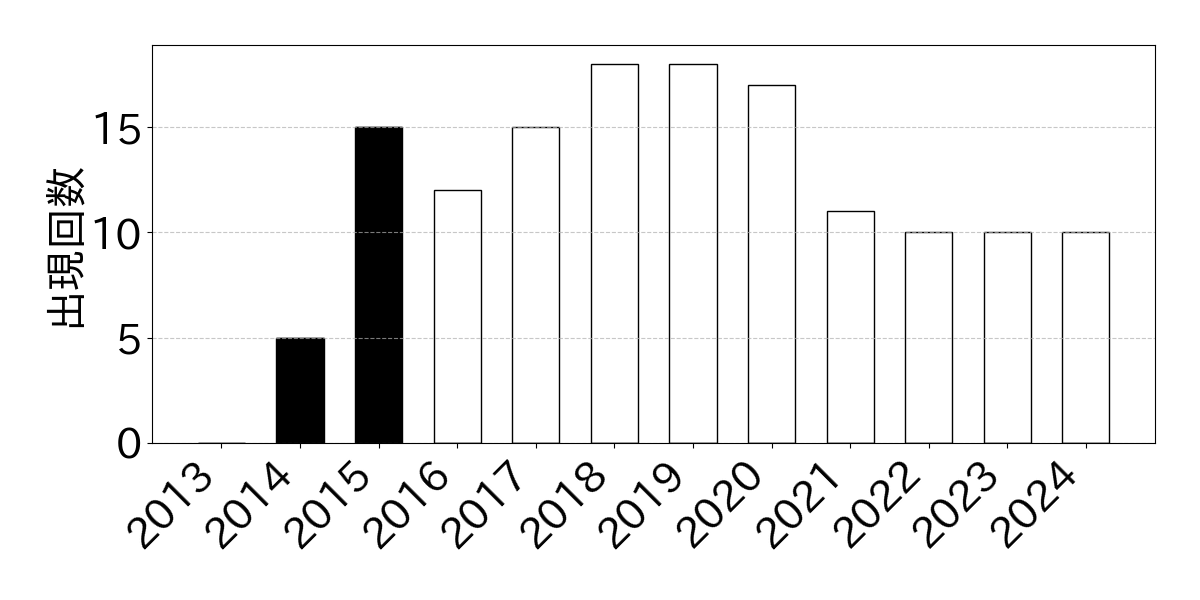
\includegraphics[width=0.8\linewidth]{@BSthesis2024_Noguchi/Noguchi_fig/id_5.png}
        \caption{id\_5のパターン}
        \label{table:id_5}

        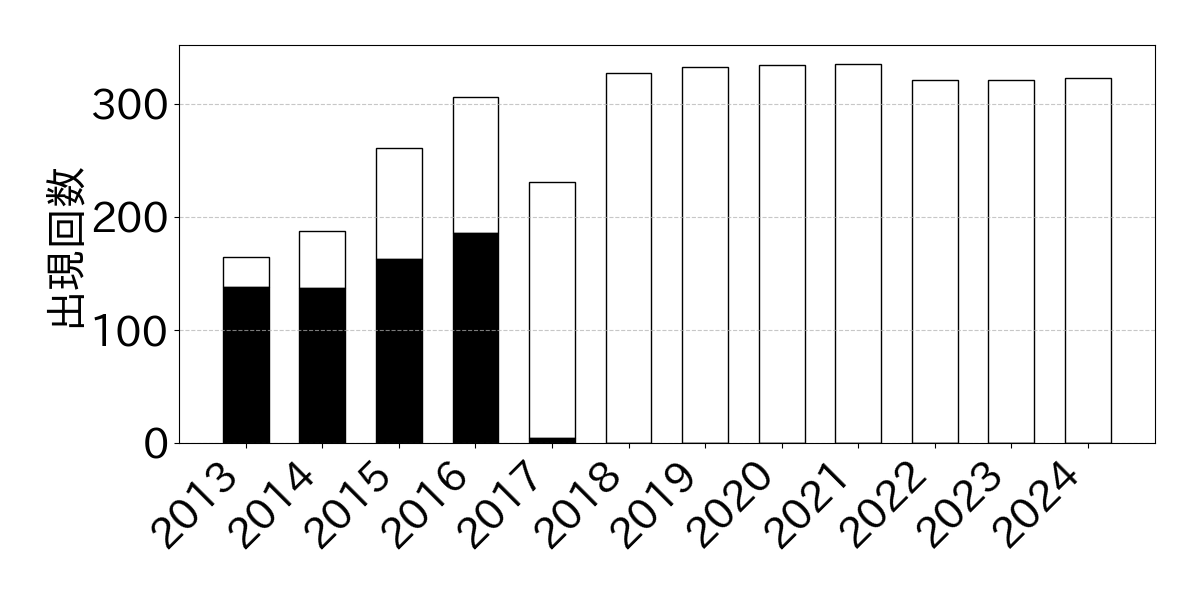
\includegraphics[width=0.8\linewidth]{@BSthesis2024_Noguchi/Noguchi_fig/id_6.png}
        \caption{id\_6のパターン}
        \label{table:id_6}
\end{figure}

当該パターンに該当するid\_2,id\_5,id\_6は,ある時点を境に,変更前パターンから完全に変更後パターンに置き換えられている.これらのパターンは,従来の記述方法を関数化することで再利用性を高めている.これらのパターンは,再利用性を重視したソースコードの実装方法がプロジェクト内で広く採用された結果であると考えられる.関数化によってコードの重複を減らし,保守性を向上させる効果があったため,これらのパターンは継続的に使用するべきパターンであると考えられる.なお,コード自動修正技術における多様なプログラミング言語を学習した深層学習では,このようなパターンの自動修正は難しいと考える.

\noindent\textbf{[消失型パターン] }


当該パターンに該当するid\_4は,図\ref{table:id_4}より,2021年を境に変更前/変更後パターンの両方が出現しなくなっている.このパターンは,ログメッセージを異なる言語で翻訳して出力するための変更である.変更前パターンで使用される`\texttt{\_}'は,一般的なローカライズ関数で,変更後パターンでは,ログ専用のローカライズ関数である`\texttt{\_LI}'などが用いられていた.ローカライズを明確にすることで,メッセージ管理や保守性を向上させるための修正方法である.

しかし,このパターンは\texttt{Python}の標準モジュールである\texttt{logging}を用いて実装されたソースコードに基づいている.\texttt{logging}モジュールは,\texttt{Python3.2}以降翻訳関数を使用せず,引数を追加することでログメッセージの翻訳をより効率的に行えるようになった.そのため,id\_4のパターンは2021年を境に使われなくなったと考えられる.従って,消失型パターンは,プログラミング言語と密接に関連しているため,結果的に不要になった,または新たな実装方法へと置き換えられた可能性が高いと考えられる.

\begin{figure}[h]
    \centering
        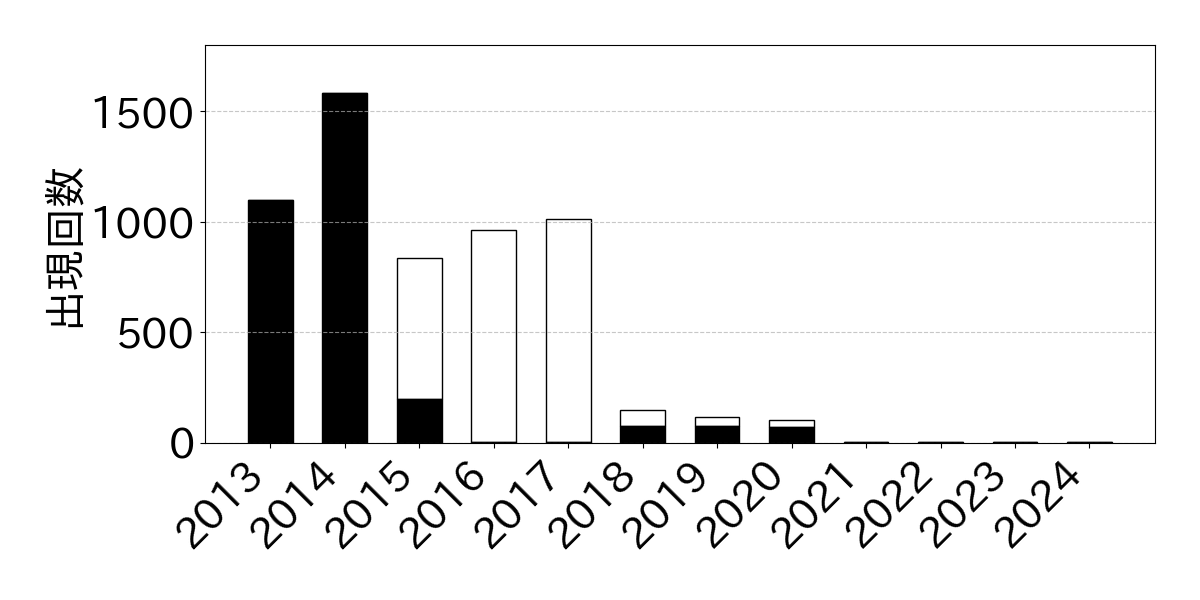
\includegraphics[width=0.8\linewidth]{@BSthesis2024_Noguchi/Noguchi_fig/id_4.png}
        \vspace{-4mm}
        \caption{id\_4のパターン}
        \label{table:id_4}
\end{figure}

%%%%%%%%%%%%%%%%%%%%%%%%%%%%%%%%%%%%%%%%%%
\chapter{妥当性の脅威}
%%%%%%%%%%%%%%%%%%%%%%%%%%%%%%%%%%%%%%%%%%
\section{内的妥当性}
コーディングパターン候補を生成する際に使用した手法について議論する.本研究で使用したPrefixSpanアルゴリズムは,頻出系列パターンを効率的に抽出する手法であり,特に大規模なデータセットに対して,高い性能を有する.今回の研究対象である12年間にわたる大規模なデータセットに対して,頻出するコードパターンを探索する上で適切な選択であるといえる.

さらに,本研究では,パターンとして採用するトークン長を最大15に制限した.この制限は,PrefixSpanによる探索時間の膨張を防止するための措置である.また,対象とした変更差分が行単位の比較的短い変更であることから,長いトークン系列はプロジェクト内で頻出しにくい.従って,トークン長に制限を設けることで分析の焦点がより妥当な範囲に絞られ,効率的かつ実用的なパターン抽出が可能となったと考えられる.
\section{外的妥当性}
本研究では,データセットとして,OpenStackのコンポーネントの中で,最大規模のプロジェクトであるNovaプロジェクト内のPythonファイルを対象に修正方法を収集し,分析を行った.本論文の手法は,バージョン管理ツールを利用し,変更チャンクを取得できるプロジェクトであれば,Python以外の言語を使用するプロジェクトにも同様に適用可能である.従って,本手法は他のプログラミング言語を用いたプロジェクトを対象とした場合でも,有効な分析結果が得られる可能性が高い.特に,異なるプロジェクトに適用することで,各プロジェクトに特有の実装方法や設計手法の違いに関する新たな知見が得られることが期待される.これにより,修正方法やパターンの普遍性の検証,さらなる適用領域の拡張につながる可能性がある.
%%%%%%%%%%%%%%%%%%%%%%%%%%%%%%%%%%%%%%%%%%
\chapter{おわりに}
%%%%%%%%%%%%%%%%%%%%%%%%%%%%%%%%%%%%%%%%%%
本研究では,個別のプロジェクトに特化したコーディングパターンを収集するための条件を提案することで,自動修正に有用なパターンを抽出する方法を開発し,2つのRQを検証した.
\begin{itemize}
    \item RQ1: \RQone
    \item RQ2: \RQtwo
\end{itemize}
RQ1の検証では,従来手法のパターン除外条件を再設計することにより,プロジェクト固有のコーディングパターンをより広範に収集することに成功した.具体的には,従来手法では除外されていた引数の追加・削除といった変更パターンの抽出を可能とし,同時に冗長なパターンの除去も実現した.

RQ2の検証においては,コーディングパターンの持続性分析を通じて,効果的なパターン収集方法の確立を試みた.分析の結果,パターンは以下の3種類に分類された.
\begin{itemize}
    \item 分析期間を通じて変更前/変更後パターンが継続的に共存する持続共存型パターン
    \item ある時点を境に,変更前パターンが完全に変更後パターンに置き換えられた移行完了型パターン
    \item ある時点で,変更前/変更後パターンが出現しなくなった消失型パターン
\end{itemize}

特に,移行完了型パターンは,プロジェクト独自に定義された関数への変更を含むケースが多く,多様なプログラミング言語を学習した深層学習モデルでは対応が困難な性質を持つことが明らかとなった.このことから,移行完了型パターンは本研究で定義するコーディングパターンとして特に重要な意義を持つと結論付けられる.

本研究で提案した手法は,プロジェクトの変更履歴から抽出したコーディングパターン候補に対して,有用性に基づく選別を行うことで,対象プロジェクト固有の修正パターンの発見を可能にした.この成果は,従来の汎用的な深層学習アプローチでは対応が困難であった修正パターンの抽出を実現するものであり,プロジェクト特化型の自動修正技術に活用できることが示唆される.
%%%%%%%%%%%%%%%%%%%%%%%%%%%%%%%%%%%%%%%%%%%%%%%%%%%%%%%%%%%%%%%%%%%%%%%%

%%
%% 謝辞
%%
\begin{acknowledgements}
本研究を進めるにあたり,多くの方々にご指導,ご協力,ご支援を賜りました.ここにお世話になった方々への感謝の意を記させていただきます.

はじめに,指導教員である和歌山大学システム工学部の伊原彰紀准教授に深く御礼申し上げます.研究室配属以来,研究方針についての相談や論文執筆,発表資料の作成など,多くの時間を割いてご指導いただきました.特に,対外発表の機会を設けていただいたことで,研究の面白さや難しさ,やりがいを知ることができ,研究に対する知見を深めることができました.先生のご尽力に敬意を表し,心より感謝いたします.

次に,和歌山大学システム工学研究科を修了された大森楓己氏並びに同研究科の亀岡令氏,そしてソーシャルソフトウェア工学研究室の先輩方には,研究において多くのご指導とご助言をいただきました.お忙しい中,研究内容の相談や論文執筆についての支援など,大変お世話になりました.心より感謝いたします.

また,和歌山大学ソーシャルソフトウェア工学研究室の皆様には,研究に関する客観的なご意見やご指導を常日頃から多くいただきました.特に同期の皆様には,研究活動のみならず,大学生活全般においても大変お世話になりました.心より感謝申し上げます.

最後に,日頃から温かく見守ってくれた家族に心より感謝いたします.
% %-------------------
% \begin{center}
% \includegraphics[width=1.0\linewidth]{@BSthesis2024_Noguchi/Noguchi_fig/thank_irasutoya.pdf}
% \end{center}
% %-------------------

\end{acknowledgements}

%%%%%%%%%%%%%%%%%%%%%%%%%%%%%%%%%%%%%%%%%%
%% 参考文献
%%%%%%%%%%%%%%%%%%%%%%%%%%%%%%%%%%%%%%%%%%
\bibliographystyle{junsrt}
\bibliography{@BSthesis2024_Noguchi/BSthesis2024_Noguchi_thesis}

\end{document}
